\documentclass{standalone}
\usepackage{tikz}
\usetikzlibrary{patterns, positioning}


\begin{document}
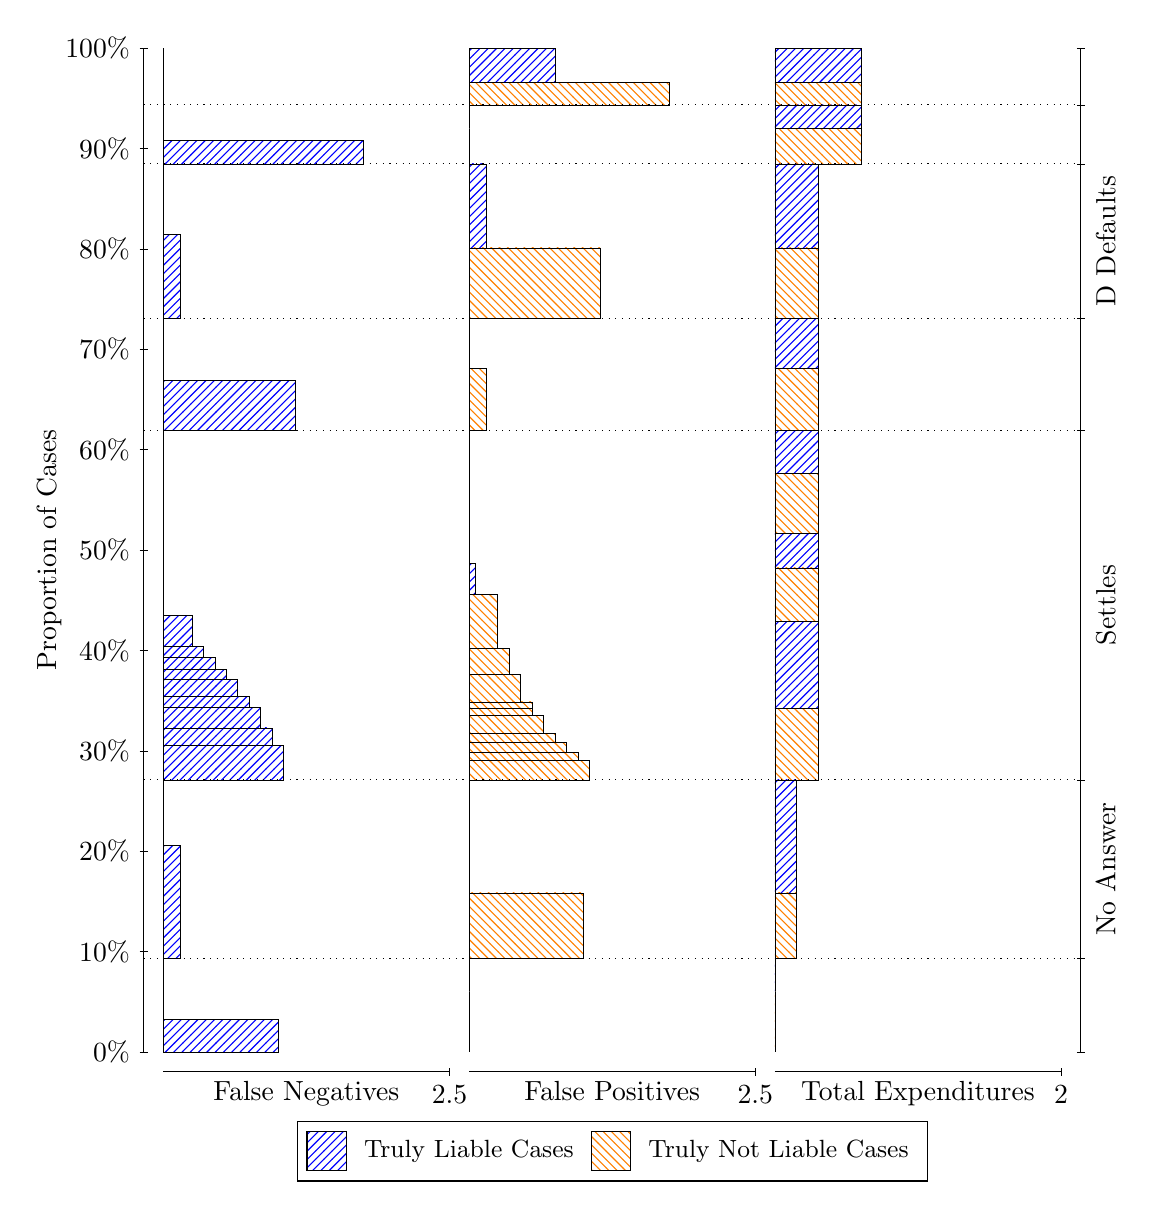
\begin{tikzpicture}
\draw[black, very thin] (1.5,1.75) -- (1.5,14.5);
\node[rotate=90, text=black, anchor=center] at (0.3, 8.125) {Proportion of Cases};
\draw[black, very thin] (1.45,1.75) -- (1.55,1.75);
\node[text=black, anchor=east] at (1.45, 1.75) {0\%};
\draw[black, very thin] (1.45,3.025) -- (1.55,3.025);
\node[text=black, anchor=east] at (1.45, 3.025) {10\%};
\draw[black, very thin] (1.45,4.3) -- (1.55,4.3);
\node[text=black, anchor=east] at (1.45, 4.3) {20\%};
\draw[black, very thin] (1.45,5.575) -- (1.55,5.575);
\node[text=black, anchor=east] at (1.45, 5.575) {30\%};
\draw[black, very thin] (1.45,6.85) -- (1.55,6.85);
\node[text=black, anchor=east] at (1.45, 6.85) {40\%};
\draw[black, very thin] (1.45,8.125) -- (1.55,8.125);
\node[text=black, anchor=east] at (1.45, 8.125) {50\%};
\draw[black, very thin] (1.45,9.4) -- (1.55,9.4);
\node[text=black, anchor=east] at (1.45, 9.4) {60\%};
\draw[black, very thin] (1.45,10.675) -- (1.55,10.675);
\node[text=black, anchor=east] at (1.45, 10.675) {70\%};
\draw[black, very thin] (1.45,11.95) -- (1.55,11.95);
\node[text=black, anchor=east] at (1.45, 11.95) {80\%};
\draw[black, very thin] (1.45,13.225) -- (1.55,13.225);
\node[text=black, anchor=east] at (1.45, 13.225) {90\%};
\draw[black, very thin] (1.45,14.5) -- (1.55,14.5);
\node[text=black, anchor=east] at (1.45, 14.5) {100\%};

\draw[black, very thin] (13.4,1.75) -- (13.4,14.5);
\draw[black, very thin] (13.35,1.75) -- (13.45,1.75);
\node[anchor=west] at (13.35, 1.75) {};
\draw[black, very thin] (13.35,2.9361) -- (13.45,2.9361);
\node[anchor=west] at (13.35, 2.9361) {};
\draw[black, very thin] (13.35,5.2059) -- (13.45,5.2059);
\node[anchor=west] at (13.35, 5.2059) {};
\draw[black, very thin] (13.35,9.6482) -- (13.45,9.6482);
\node[anchor=west] at (13.35, 9.6482) {};
\draw[black, very thin] (13.35,11.07) -- (13.45,11.07);
\node[anchor=west] at (13.35, 11.07) {};
\draw[black, very thin] (13.35,13.029) -- (13.45,13.029);
\node[anchor=west] at (13.35, 13.029) {};
\draw[black, very thin] (13.35,13.778) -- (13.45,13.778);
\node[anchor=west] at (13.35, 13.778) {};
\draw[black, very thin] (13.35,14.5) -- (13.45,14.5);
\node[anchor=west] at (13.35, 14.5) {};

\draw[black, very thin, pattern color=blue, pattern=north east lines] (1.75,1.75) rectangle (3.2033,2.168);
\draw[black, very thin, pattern color=orange, pattern=north west lines] (1.75,2.168) rectangle (1.75,2.9361);
\draw[black, very thin, pattern color=blue, pattern=north east lines] (1.75,2.9361) rectangle (1.968,4.3703);
\draw[black, very thin, pattern color=orange, pattern=north west lines] (1.75,4.3703) rectangle (1.75,5.2059);
\draw[black, very thin, pattern color=blue, pattern=north east lines] (1.75,5.2059) rectangle (3.276,5.6411);
\draw[black, very thin, pattern color=blue, pattern=north east lines] (1.75,5.6411) rectangle (3.1307,5.8647);
\draw[black, very thin, pattern color=blue, pattern=north east lines] (1.75,5.8647) rectangle (2.9853,6.1241);
\draw[black, very thin, pattern color=blue, pattern=north east lines] (1.75,6.1241) rectangle (2.84,6.2706);
\draw[black, very thin, pattern color=blue, pattern=north east lines] (1.75,6.2706) rectangle (2.6947,6.4841);
\draw[black, very thin, pattern color=blue, pattern=north east lines] (1.75,6.4841) rectangle (2.5493,6.6049);
\draw[black, very thin, pattern color=blue, pattern=north east lines] (1.75,6.6049) rectangle (2.404,6.7633);
\draw[black, very thin, pattern color=blue, pattern=north east lines] (1.75,6.7633) rectangle (2.2587,6.8971);
\draw[black, very thin, pattern color=blue, pattern=north east lines] (1.75,6.8971) rectangle (2.1133,7.2966);
\draw[black, very thin, pattern color=orange, pattern=north west lines] (1.75,7.2966) rectangle (1.75,9.6482);
\draw[black, very thin, pattern color=blue, pattern=north east lines] (1.75,9.6482) rectangle (3.4213,10.282);
\draw[black, very thin, pattern color=orange, pattern=north west lines] (1.75,10.282) rectangle (1.75,11.07);
\draw[black, very thin, pattern color=blue, pattern=north east lines] (1.75,11.07) rectangle (1.968,12.137);
\draw[black, very thin, pattern color=orange, pattern=north west lines] (1.75,12.137) rectangle (1.75,13.029);
\draw[black, very thin, pattern color=blue, pattern=north east lines] (1.75,13.029) rectangle (4.2933,13.326);
\draw[black, very thin, pattern color=orange, pattern=north west lines] (1.75,13.326) rectangle (1.75,13.778);
\draw[black, very thin, pattern color=orange, pattern=north west lines] (1.75,13.778) rectangle (1.75,14.066);
\draw[black, very thin, pattern color=blue, pattern=north east lines] (1.75,14.066) rectangle (1.75,14.5);
\draw[black, very thin, pattern color=orange, pattern=north west lines] (5.6333,1.75) rectangle (5.6333,2.5181);
\draw[black, very thin, pattern color=blue, pattern=north east lines] (5.6333,2.5181) rectangle (5.6333,2.9361);
\draw[black, very thin, pattern color=orange, pattern=north west lines] (5.6333,2.9361) rectangle (7.0867,3.7716);
\draw[black, very thin, pattern color=blue, pattern=north east lines] (5.6333,3.7716) rectangle (5.6333,5.2059);
\draw[black, very thin, pattern color=orange, pattern=north west lines] (5.6333,5.2059) rectangle (7.1593,5.454);
\draw[black, very thin, pattern color=orange, pattern=north west lines] (5.6333,5.454) rectangle (7.014,5.5546);
\draw[black, very thin, pattern color=orange, pattern=north west lines] (5.6333,5.5546) rectangle (6.8687,5.683);
\draw[black, very thin, pattern color=orange, pattern=north west lines] (5.6333,5.683) rectangle (6.7233,5.7982);
\draw[black, very thin, pattern color=orange, pattern=north west lines] (5.6333,5.7982) rectangle (6.578,6.0229);
\draw[black, very thin, pattern color=orange, pattern=north west lines] (5.6333,6.0229) rectangle (6.4327,6.1152);
\draw[black, very thin, pattern color=orange, pattern=north west lines] (5.6333,6.1152) rectangle (6.4327,6.1956);
\draw[black, very thin, pattern color=orange, pattern=north west lines] (5.6333,6.1956) rectangle (6.2873,6.5469);
\draw[black, very thin, pattern color=orange, pattern=north west lines] (5.6333,6.5469) rectangle (6.142,6.8774);
\draw[black, very thin, pattern color=orange, pattern=north west lines] (5.6333,6.8774) rectangle (5.9967,7.5574);
\draw[black, very thin, pattern color=blue, pattern=north east lines] (5.6333,7.5574) rectangle (5.706,7.957);
\draw[black, very thin, pattern color=blue, pattern=north east lines] (5.6333,7.957) rectangle (5.6333,9.6482);
\draw[black, very thin, pattern color=orange, pattern=north west lines] (5.6333,9.6482) rectangle (5.8513,10.436);
\draw[black, very thin, pattern color=blue, pattern=north east lines] (5.6333,10.436) rectangle (5.6333,11.07);
\draw[black, very thin, pattern color=orange, pattern=north west lines] (5.6333,11.07) rectangle (7.3047,11.961);
\draw[black, very thin, pattern color=blue, pattern=north east lines] (5.6333,11.961) rectangle (5.8513,13.029);
\draw[black, very thin, pattern color=orange, pattern=north west lines] (5.6333,13.029) rectangle (5.6333,13.481);
\draw[black, very thin, pattern color=blue, pattern=north east lines] (5.6333,13.481) rectangle (5.6333,13.778);
\draw[black, very thin, pattern color=orange, pattern=north west lines] (5.6333,13.778) rectangle (8.1767,14.066);
\draw[black, very thin, pattern color=blue, pattern=north east lines] (5.6333,14.066) rectangle (6.7233,14.5);
\draw[black, very thin, pattern color=orange, pattern=north west lines] (9.5167,1.75) rectangle (9.5167,2.5181);
\draw[black, very thin, pattern color=blue, pattern=north east lines] (9.5167,2.5181) rectangle (9.5167,2.9361);
\draw[black, very thin, pattern color=orange, pattern=north west lines] (9.5167,2.9361) rectangle (9.7892,3.7716);
\draw[black, very thin, pattern color=blue, pattern=north east lines] (9.5167,3.7716) rectangle (9.7892,5.2059);
\draw[black, very thin, pattern color=orange, pattern=north west lines] (9.5167,5.2059) rectangle (10.062,6.1152);
\draw[black, very thin, pattern color=blue, pattern=north east lines] (9.5167,6.1152) rectangle (10.062,7.2185);
\draw[black, very thin, pattern color=orange, pattern=north west lines] (9.5167,7.2185) rectangle (10.062,7.8985);
\draw[black, very thin, pattern color=blue, pattern=north east lines] (9.5167,7.8985) rectangle (10.062,8.3338);
\draw[black, very thin, pattern color=orange, pattern=north west lines] (9.5167,8.3338) rectangle (10.062,9.0959);
\draw[black, very thin, pattern color=blue, pattern=north east lines] (9.5167,9.0959) rectangle (10.062,9.6482);
\draw[black, very thin, pattern color=orange, pattern=north west lines] (9.5167,9.6482) rectangle (10.062,10.436);
\draw[black, very thin, pattern color=blue, pattern=north east lines] (9.5167,10.436) rectangle (10.062,11.07);
\draw[black, very thin, pattern color=orange, pattern=north west lines] (9.5167,11.07) rectangle (10.062,11.961);
\draw[black, very thin, pattern color=blue, pattern=north east lines] (9.5167,11.961) rectangle (10.062,13.029);
\draw[black, very thin, pattern color=orange, pattern=north west lines] (9.5167,13.029) rectangle (10.607,13.481);
\draw[black, very thin, pattern color=blue, pattern=north east lines] (9.5167,13.481) rectangle (10.607,13.778);
\draw[black, very thin, pattern color=orange, pattern=north west lines] (9.5167,13.778) rectangle (10.607,14.066);
\draw[black, very thin, pattern color=blue, pattern=north east lines] (9.5167,14.066) rectangle (10.607,14.5);
\draw[black, dotted] (1.5,2.9361) -- (13.4,2.9361);
\draw[black, dotted] (1.5,5.2059) -- (13.4,5.2059);
\draw[black, dotted] (1.5,9.6482) -- (13.4,9.6482);
\draw[black, dotted] (1.5,11.07) -- (13.4,11.07);
\draw[black, dotted] (1.5,13.029) -- (13.4,13.029);
\draw[black, dotted] (1.5,13.778) -- (13.4,13.778);
\draw[black, very thin] (1.75,1.5) -- (5.3833,1.5);
\node[text=black, anchor=north] at (3.5667, 1.5) {False Negatives};
\draw[black, very thin] (5.3833,1.45) -- (5.3833,1.55);
\node[text=black, anchor=north] at (5.3833, 1.45) {2.5};

\draw[black, very thin] (5.6333,1.5) -- (9.2667,1.5);
\node[text=black, anchor=north] at (7.45, 1.5) {False Positives};
\draw[black, very thin] (9.2667,1.45) -- (9.2667,1.55);
\node[text=black, anchor=north] at (9.2667, 1.45) {2.5};

\draw[black, very thin] (9.5167,1.5) -- (13.15,1.5);
\node[text=black, anchor=north] at (11.333, 1.5) {Total Expenditures};
\draw[black, very thin] (13.15,1.45) -- (13.15,1.55);
\node[text=black, anchor=north] at (13.15, 1.45) {2};


\node[text=black, centered, rotate=90] at (13.72, 4.071) {No Answer};
\node[text=black, centered, rotate=90] at (13.72, 7.427) {Settles};

\node[text=black, centered, rotate=90] at (13.72, 12.049) {D Defaults};



\draw (7.449999999999999,1.5) node[draw=none] (baseCoordinate) {};
\begin{scope}[align=center]
        \matrix[scale=0.5, draw=black, below=0.5cm of baseCoordinate, nodes={draw}, column sep=0.1cm]{
            \node[rectangle, draw, minimum width=0.5cm, minimum height=0.5cm, pattern color=blue, pattern=north east lines] {}; &
            \node[draw=none, font=\small, text=black] (B) {Truly Liable Cases}; &
            \node[rectangle, draw, minimum width=0.5cm, minimum height=0.5cm, pattern color=orange, pattern=north west lines] {}; &
            \node[draw=none, font=\small, text=black] (B) {Truly Not Liable Cases}; \\
            };
\end{scope}

\end{tikzpicture}
\end{document}